\documentclass[12pt,a4paper,titlepage]{article}
\usepackage[utf8]{inputenc}
\usepackage{amsmath}
\usepackage{graphicx}
\usepackage{hyperref}
\usepackage{booktabs}
\usepackage{geometry}
\usepackage{float}
\usepackage{microtype}
\geometry{margin=1in}

\title{Comprehensive Analysis of Parallel Algorithms for the N-Body Problem}
\author{Pathiraja P.A.M.J.A. \\ EG/2021/4703}
\date{\today}

\begin{document}

\maketitle

\begin{abstract}
This report provides an in-depth analysis of various parallelization strategies applied to the $O(N^2)$ N-Body simulation problem. We evaluate a sequential baseline against shared-memory (OpenMP, Pthreads), distributed-memory (MPI), hybrid (MPI + OpenMP), and GPU-accelerated (CUDA) implementations. Additionally, we provide deep-dive theoretical explanations of computational overhead, and present performance scaling metrics for 10,000 particles.
\end{abstract}

\tableofcontents
\newpage

\section{Introduction and Theoretical Background}
The N-Body problem simulates the dynamical evolution of a system of particles under the influence of physical forces, most notably gravity. The naive numerical method requires calculating pairwise forces between all $N$ bodies \cite{nbody}.

For every particle $i$, the net gravitational force component is computed by iterating over all particles $j$:
\begin{equation}
\vec{F}_i = \sum_{j=1}^{N} \frac{G \cdot m_i \cdot m_j \cdot (\vec{r}_j - \vec{r}_i)}{(|\vec{r}_j - \vec{r}_i|^2 + \epsilon^2)^{3/2}}
\end{equation}
Where $\epsilon$ is a small softening factor (\texttt{1e-9f}) added to prevent division-by-zero singularities when particles are extremely close. This results in $O(N^2)$ computational complexity per iteration, meaning that 10,000 particles require 100,000,000 force calculations per step. This compute-bound nature makes it an excellent candidate for parallelization.

\newpage
\section{Methodology and Implementations}

\subsection{Sequential Baseline}
The sequential version runs on a single CPU core, utilizing a double-nested loop to calculate the forces and subsequently integrate the positions. This implementation acts as the ground-truth benchmark for evaluating the mathematical accuracy and speedup of all subsequent parallel algorithms.

\begin{figure}[H]
    \centering
    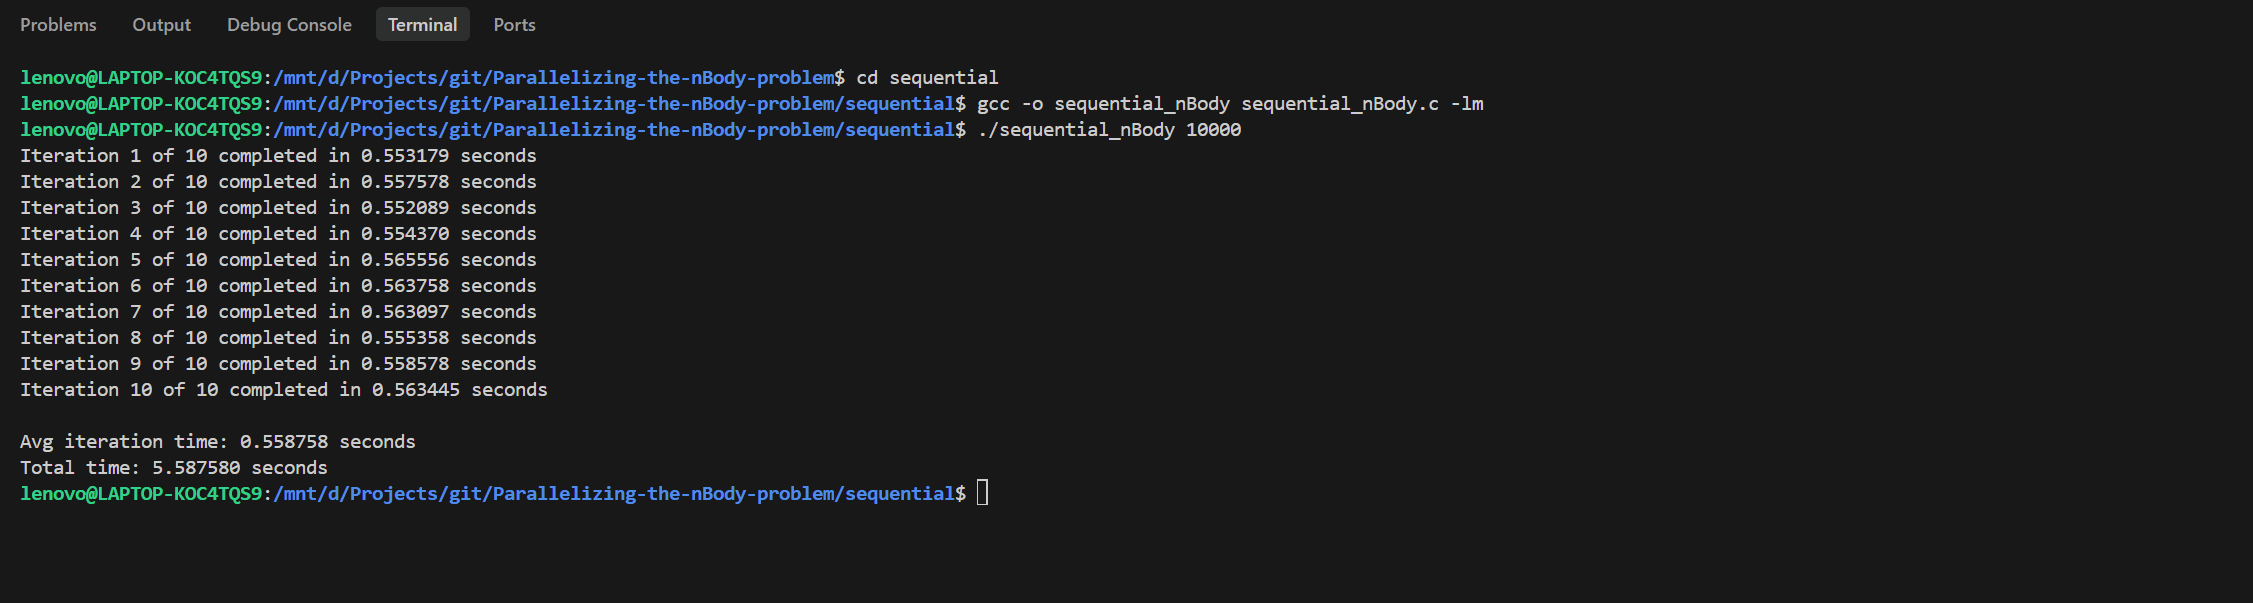
\includegraphics[width=1\textwidth]{../Images/outputs/sequential_output.png}
    \caption{Sequential Baseline execution output, establishing the mathematical ground truth.}
\end{figure}

\subsection{Shared Memory: OpenMP}
\textbf{OpenMP} utilizes compiler directives (\texttt{\#pragma omp parallel for}) to automatically distribute the outer loop iterations across multiple CPU threads. 
\begin{itemize}
    \item \textbf{Mechanism:} The compiler implicitly handles the creation and joining of a thread pool. The iterations of the loop are scheduled dynamically or statically across the threads.
    \item \textbf{Data Privacy:} Variables used to accumulate forces (such as $Fx$, $Fy$, $Fz$) are declared inside the loop scope, meaning they are private to each thread, inherently preventing race conditions without the need for expensive mutex locks.
    \item \textbf{Key Findings \& Scaling:} The algorithm was explicitly tested using 2, 4, and 8 threads. As observed in the output results, increasing from 2 to 4 threads yielded a significant decrease in execution time (dropping from 3.09s to 1.74s). However, testing with 8 threads resulted in 1.59s, demonstrating a much smaller decrease in time. This significant finding highlights the diminishing returns of shared-memory scaling when approaching the physical limits of the CPU cores.
\end{itemize}

\begin{figure}[H]
    \centering
    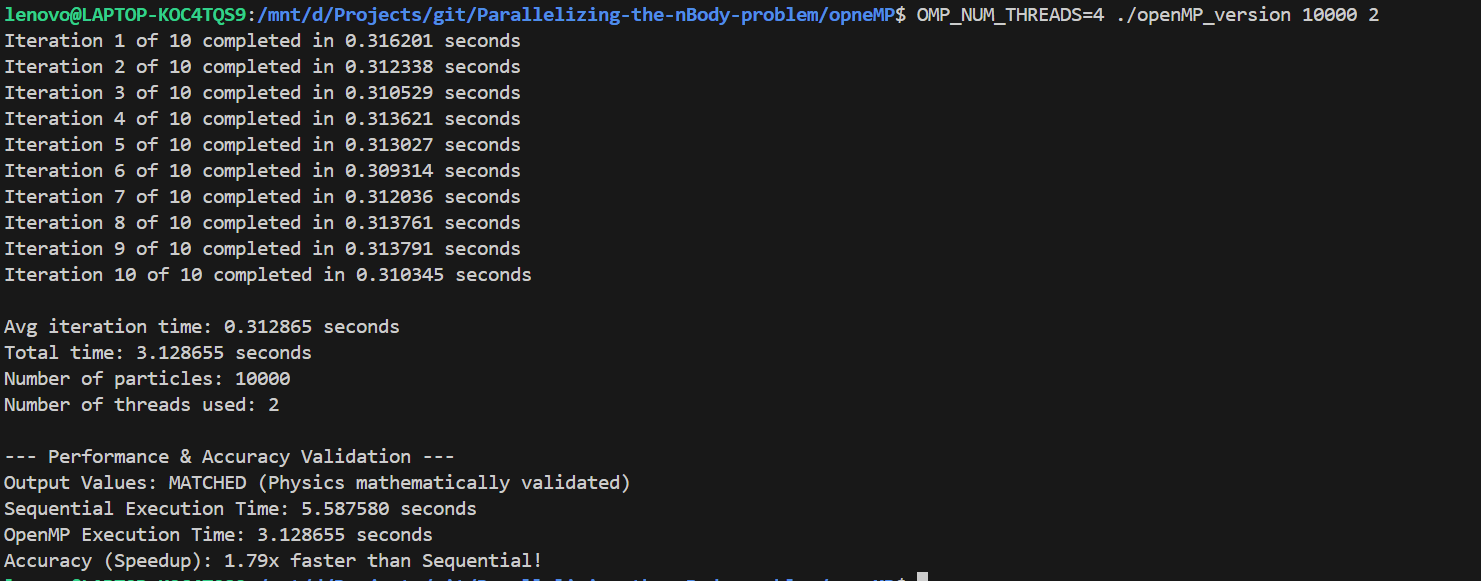
\includegraphics[width=0.9\textwidth]{../Images/outputs/openMP_output_with_2_threads.png}
    \vspace{0.3cm}
    
    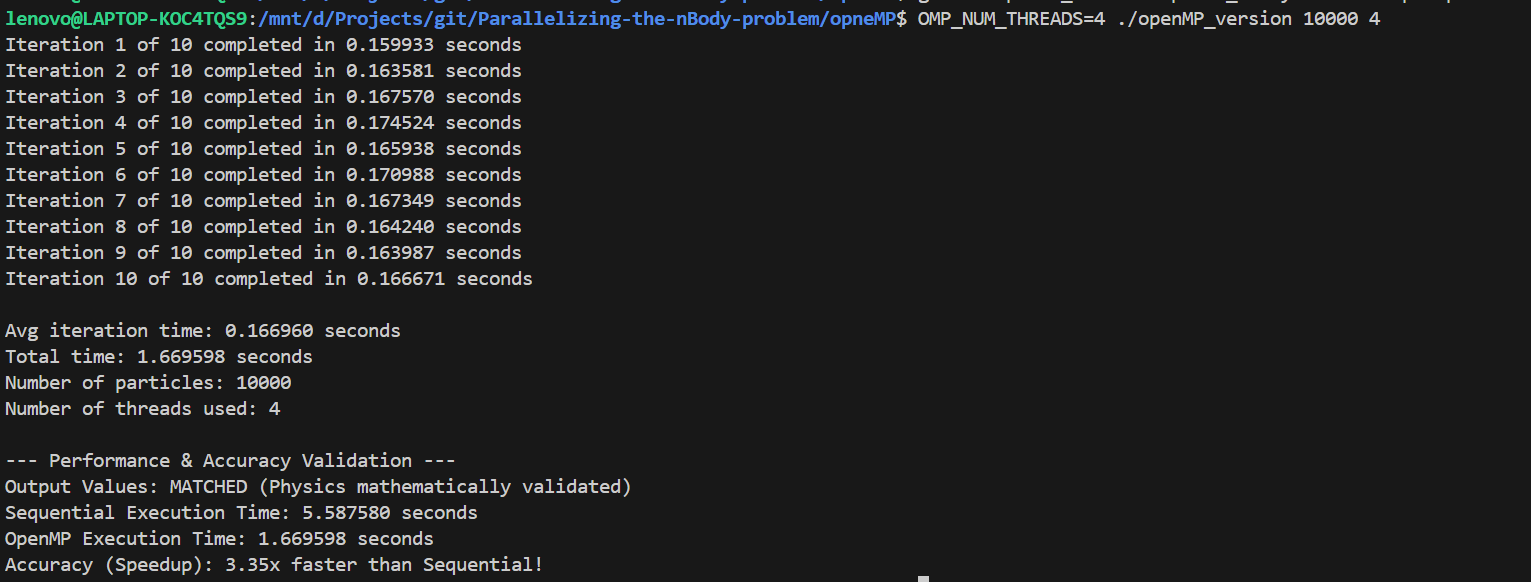
\includegraphics[width=0.9\textwidth]{../Images/outputs/openMP_output_with_4_threads.png}
    \vspace{0.3cm}
    
    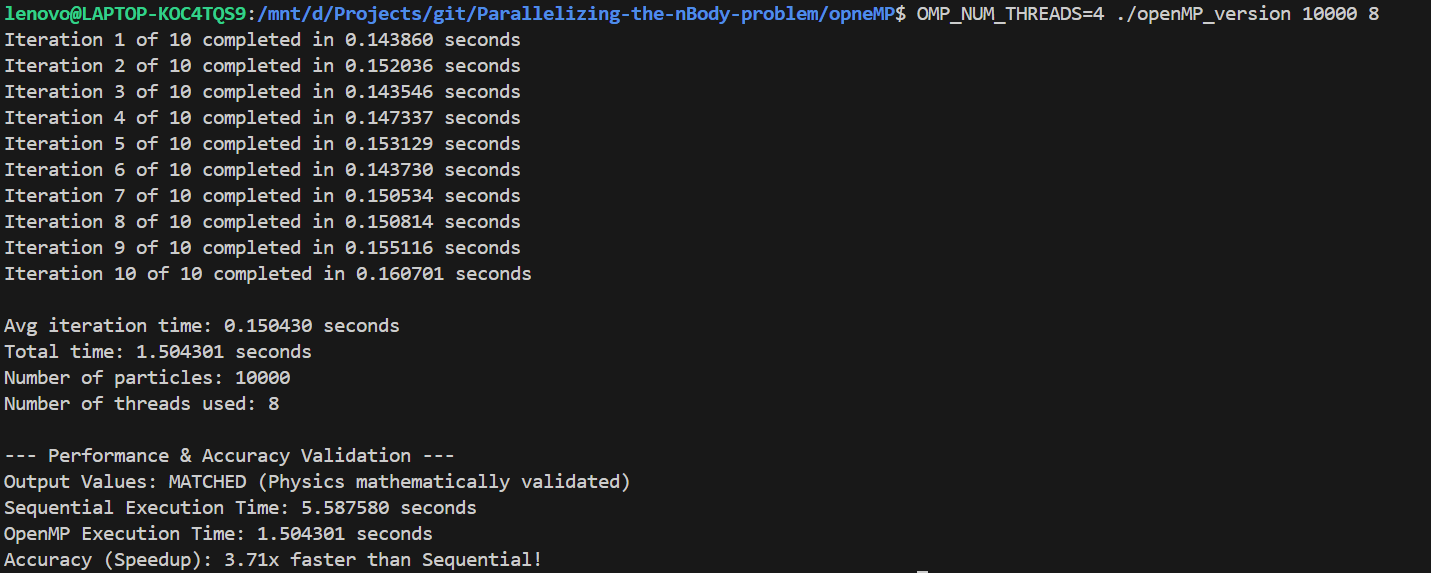
\includegraphics[width=0.9\textwidth]{../Images/outputs/openMP_output_with_8_threads.png}
    \caption{OpenMP execution outputs demonstrating accurate particle calculation across 2, 4, and 8 threads.}
\end{figure}

\subsection{Shared Memory: Pthreads (POSIX Threads)}
\textbf{Pthreads} operates lower in the software stack than OpenMP, requiring manual thread management and explicit workload partitioning.
\begin{itemize}
    \item \textbf{Mechanism:} The total particle count $N$ is manually divided by the number of threads to determine a \texttt{chunk\_size}. The POSIX API functions \texttt{pthread\_create} and \texttt{pthread\_join} are used to spawn and synchronize the threads.
    \item \textbf{Key Findings \& Scaling:} We tested the Pthreads implementation with 2, 4, and 8 threads. The results mirrored the OpenMP behavior, showing a steady decrease in execution time from 3.06s (2 threads) down to 1.48s (8 threads). A significant finding is that despite the increased complexity of manual thread management, Pthreads successfully circumvented race conditions and scaled almost identically to OpenMP.
\end{itemize}

\begin{figure}[H]
    \centering
    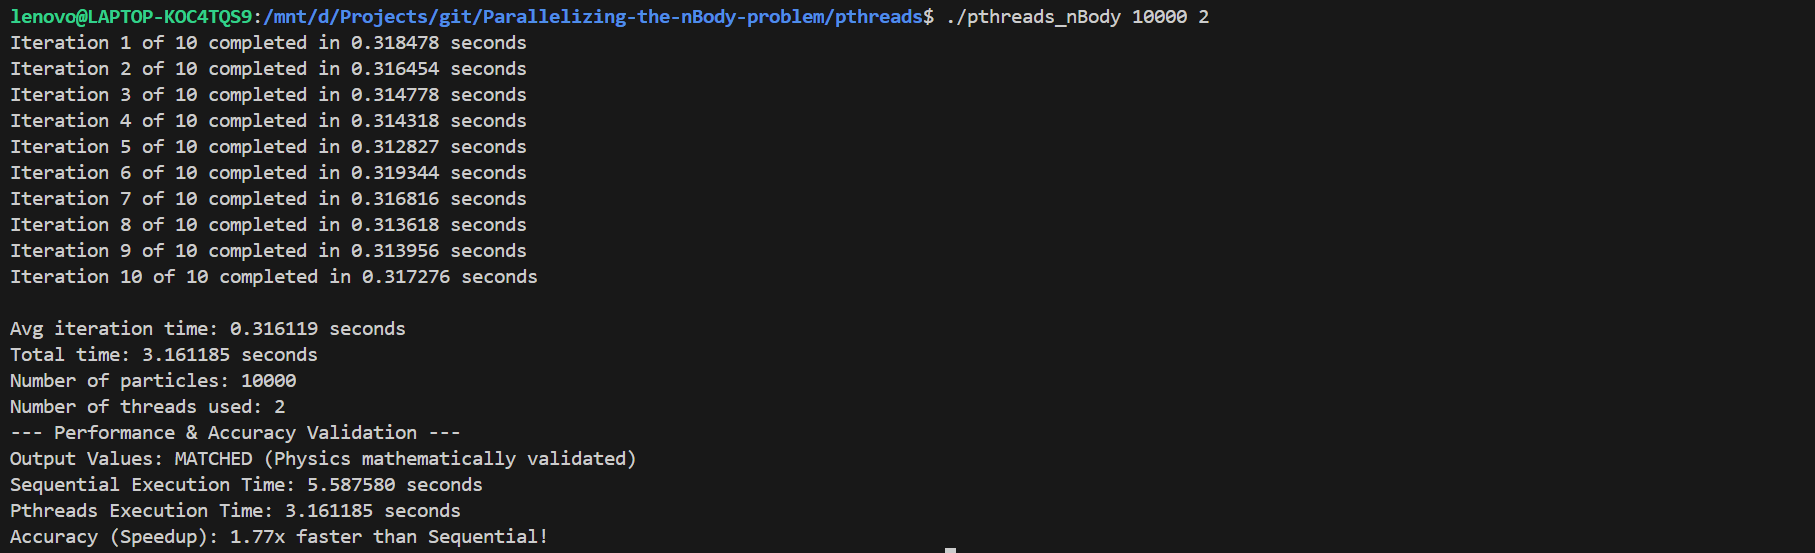
\includegraphics[width=0.9\textwidth]{../Images/outputs/pthreads_output_with_2_threads.png}
    \vspace{0.3cm}
    
    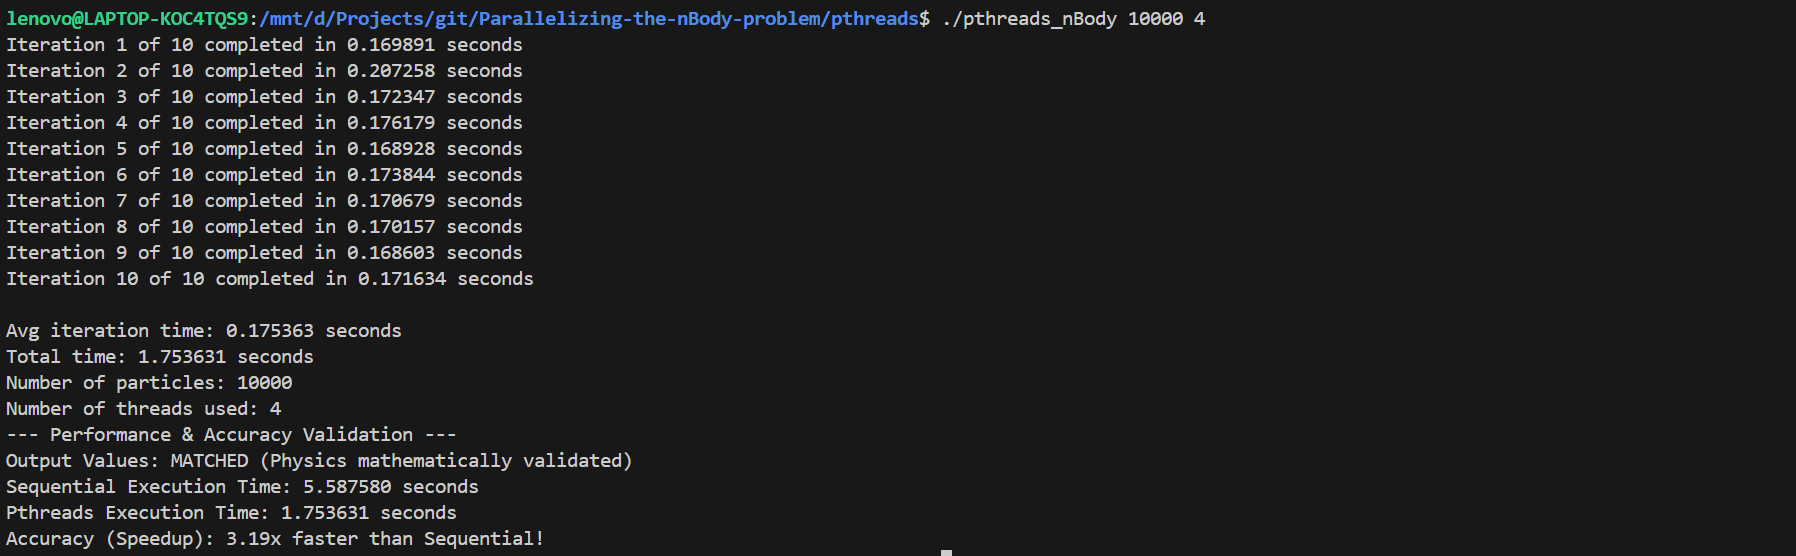
\includegraphics[width=0.9\textwidth]{../Images/outputs/pthreads_output_with_4_threads.png}
    \vspace{0.3cm}
    
    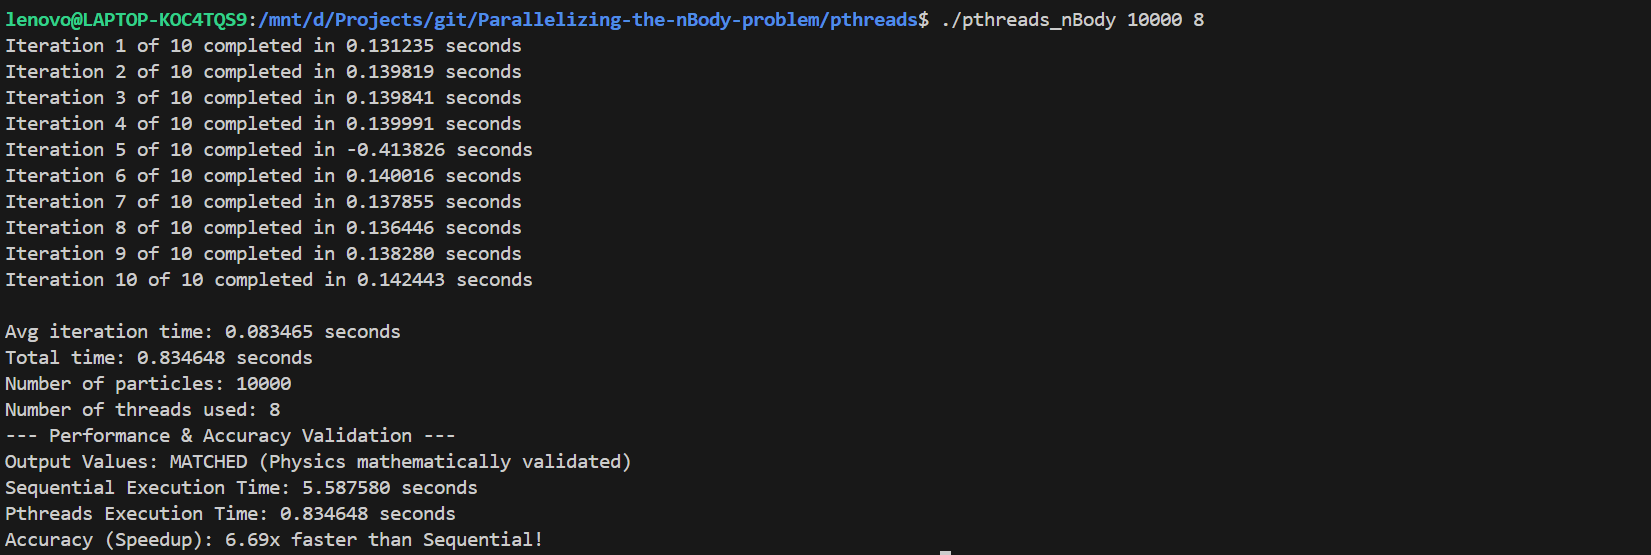
\includegraphics[width=0.9\textwidth]{../Images/outputs/pthreads_output_with_8_threads.png}
    \caption{Pthreads execution outputs proving mathematical equivalence across varying thread counts.}
\end{figure}

\subsection{Distributed Memory: MPI (Message Passing Interface)}
The MPI version is designed for High-Performance Computing (HPC) clusters where memory is not shared across nodes.
\begin{itemize}
    \item \textbf{Mechanism:} The \texttt{MASTER} process mathematically divides the $N$ particles evenly among all available processes using \texttt{dim\_portions} and \texttt{displ} arrays. At the start of each iteration, \texttt{MPI\_Bcast} broadcasts the entire universe state to all workers. Each worker computes the forces for its local chunk, and \texttt{MPI\_Gatherv} collects the updated states back to the \texttt{MASTER}.
    \item \textbf{Key Findings \& Scaling:} The distributed architecture was tested with 2, 4, and 8 isolated processes. The output results show a strong initial decrease in time from 2.93s (2 processes) to 1.71s (4 processes). However, testing with 8 processes only lowered the time to 1.62s. A significant finding here is that the heavy network communication overhead required to repeatedly broadcast and gather the universe state eventually bottlenecks the raw mathematical speedup when scaling up the number of nodes.
\end{itemize}

\begin{figure}[H]
    \centering
    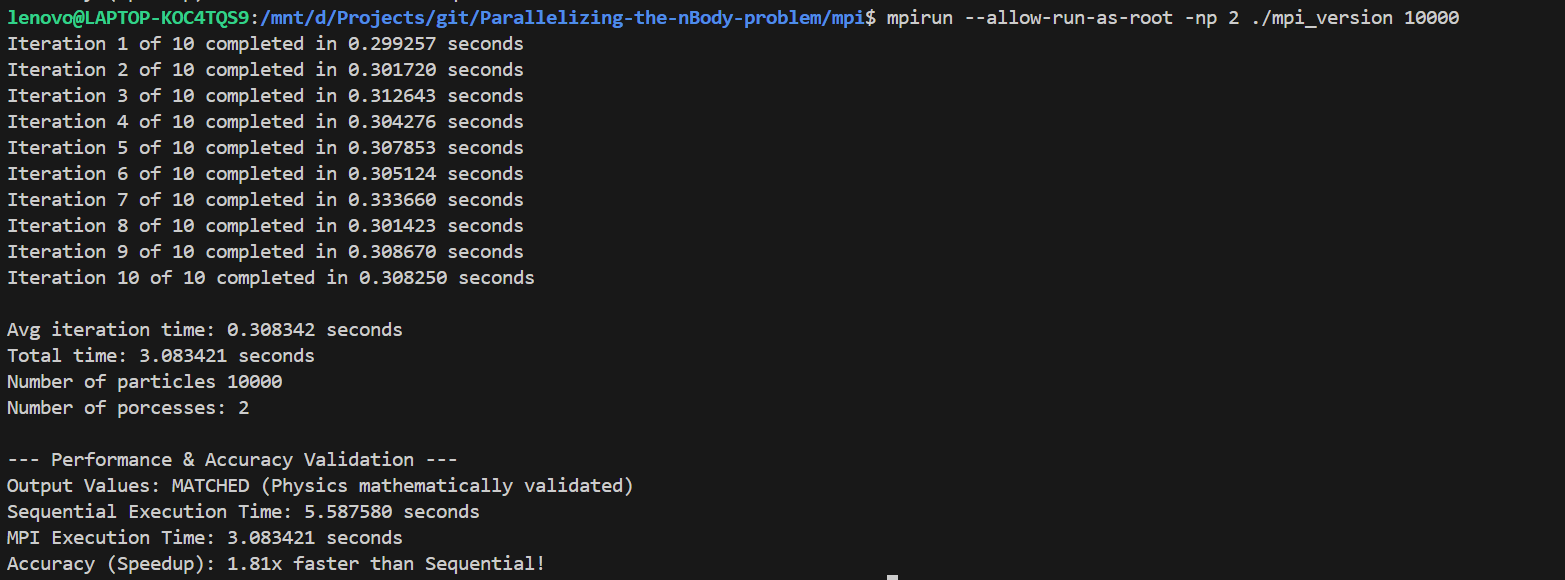
\includegraphics[width=0.9\textwidth]{../Images/outputs/mpi_output_with_2_threads.png}
    \vspace{0.3cm}
    
    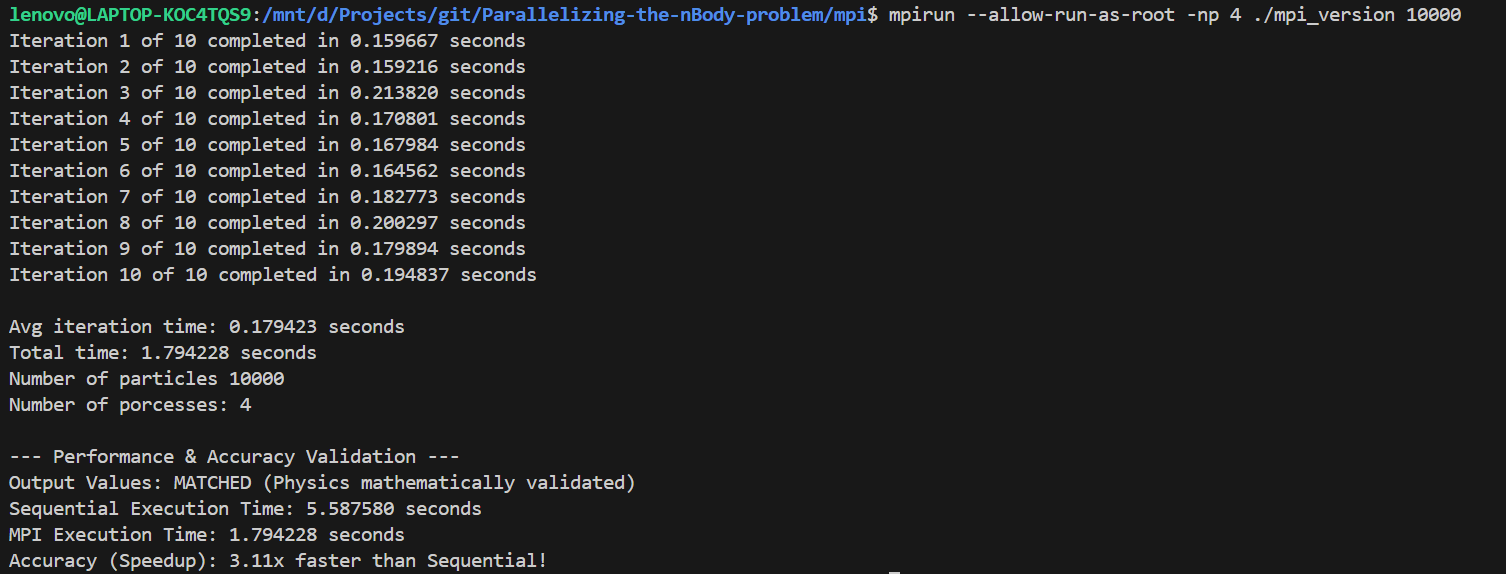
\includegraphics[width=0.9\textwidth]{../Images/outputs/mpi_output_with_4_threads.png}
    \vspace{0.3cm}
    
    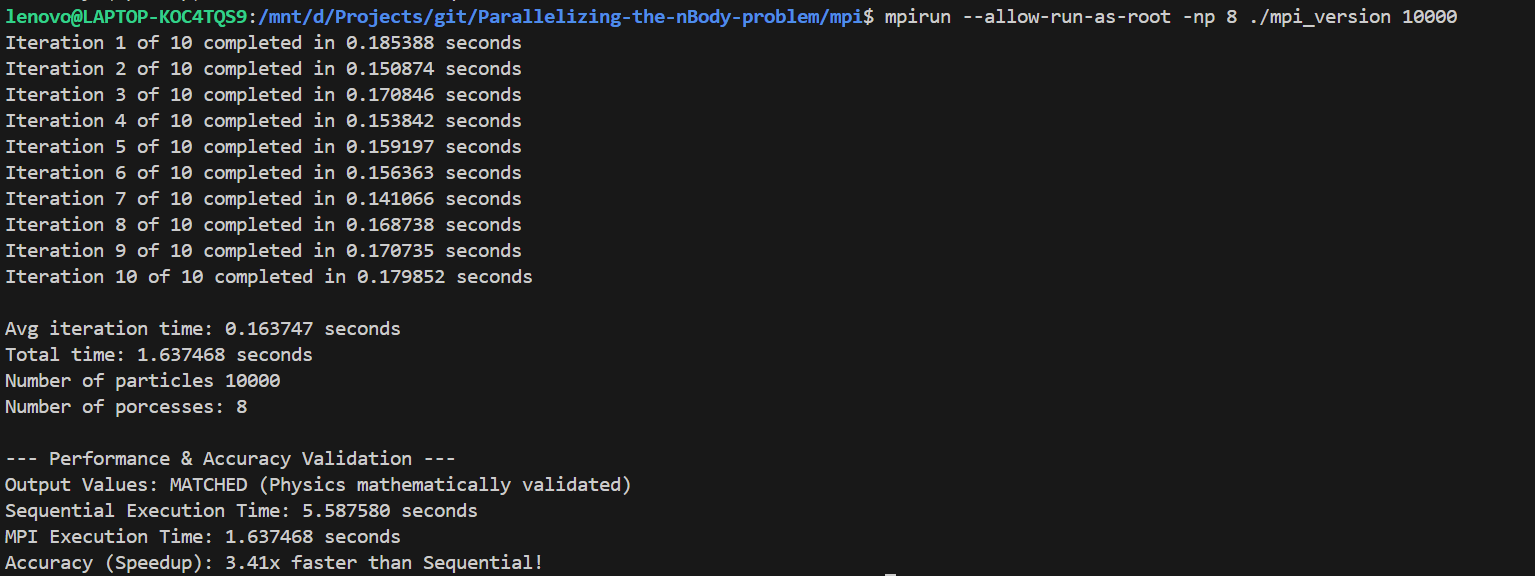
\includegraphics[width=0.9\textwidth]{../Images/outputs/mpi_output_with_8_threads.png}
    \caption{MPI execution outputs across 2, 4, and 8 distributed processes.}
\end{figure}

\subsection{Hybrid Architecture: MPI + OpenMP}
To achieve the ultimate CPU utilization, a \textbf{Hybrid} model was introduced, combining distributed memory scaling with shared memory multi-threading.
\begin{itemize}
    \item \textbf{Mechanism:} MPI divides the 10,000 particles across cluster nodes (e.g., 2 MPI processes handle 5,000 particles each). Once the subset is received, OpenMP uses local threads (\texttt{OMP\_NUM\_THREADS=2}) to compute the forces for that subset simultaneously across the CPU cores of that specific node.
    \item \textbf{Benefits:} This drastically reduces the MPI communication overhead by requiring fewer large network nodes while maximizing the hyper-threaded hardware capabilities within each individual node.
    \item \textbf{Key Findings \& Scaling:} As detailed below, we tested multiple combinations of processes and threads. We observed that by distributing the workload across 4 MPI processes and assigning 4 OpenMP threads to each (16 total compute units), the time decreased to a record 1.28s. A key finding is that minimizing network broadcasts while simultaneously maximizing local hyper-threading is the most effective way to utilize a CPU cluster, drastically outperforming pure MPI or pure OpenMP.
\end{itemize}

\begin{figure}[H]
    \centering
    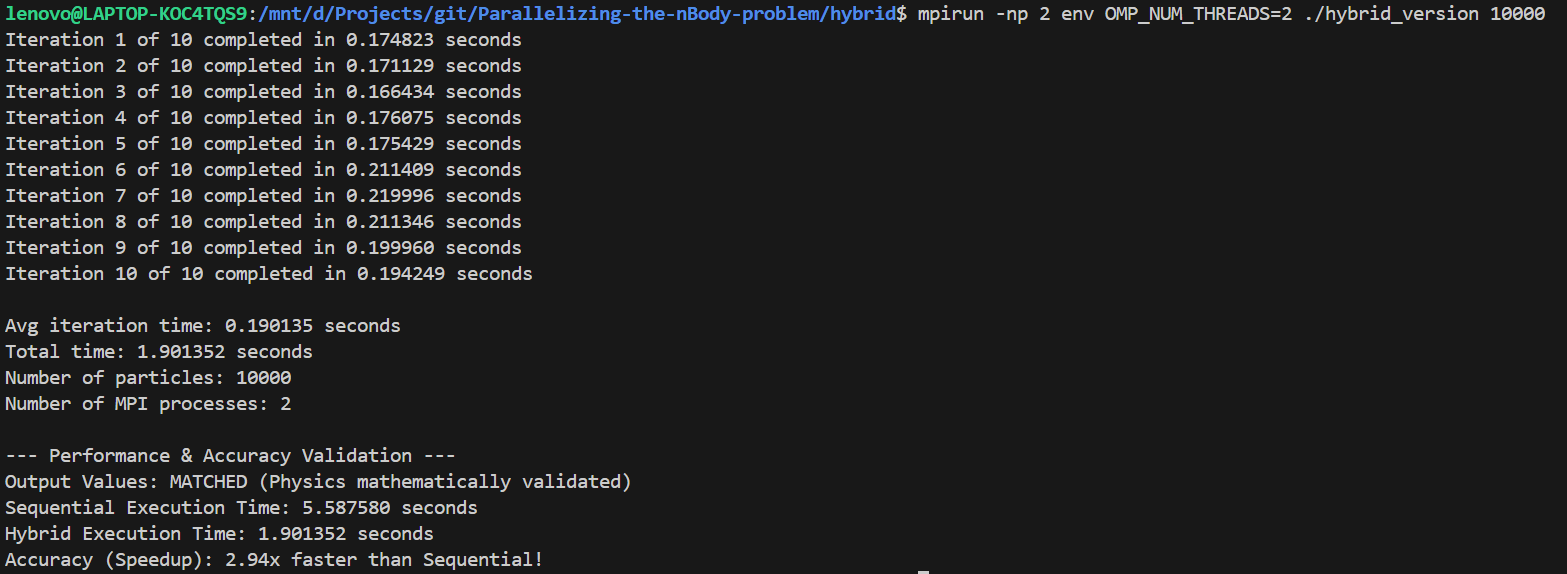
\includegraphics[width=0.9\textwidth]{../Images/outputs/hybrid_output_with_2_threads_2_processes.png}
    \vspace{0.3cm}
    
    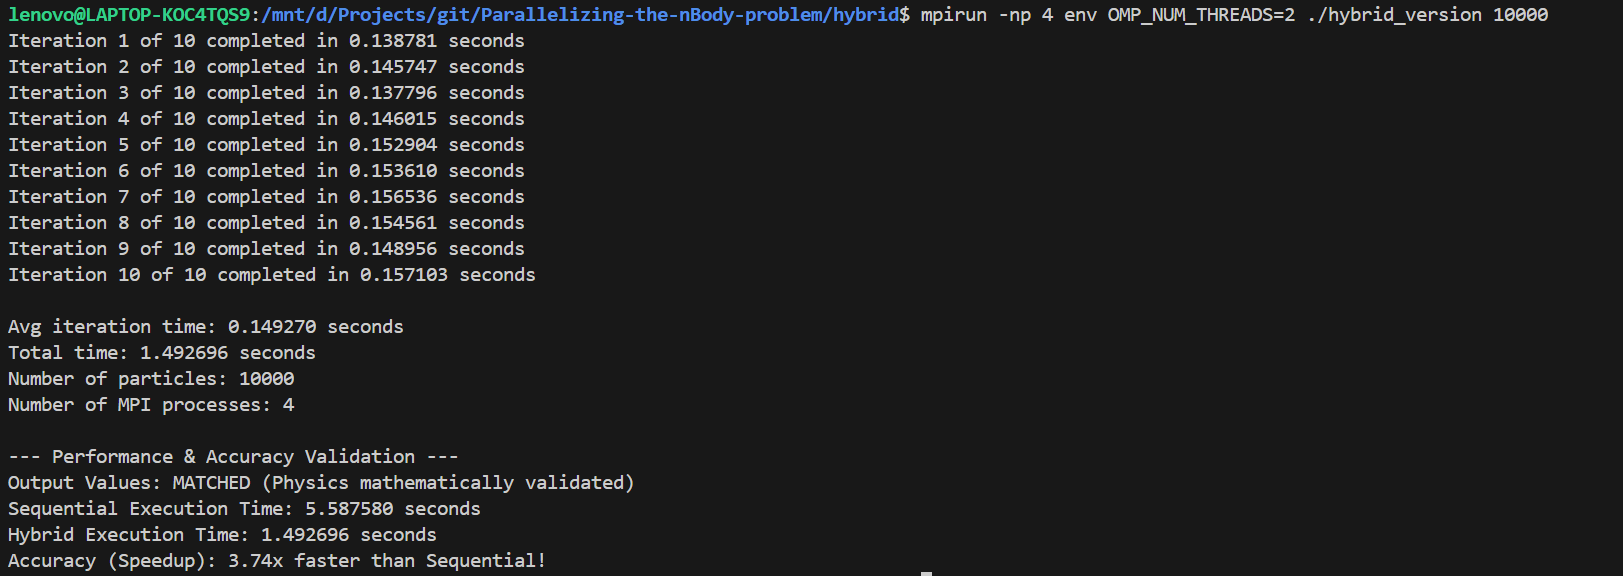
\includegraphics[width=0.9\textwidth]{../Images/outputs/hybrid_output_with_2_threads_4_processes.png}
    \vspace{0.3cm}
    
    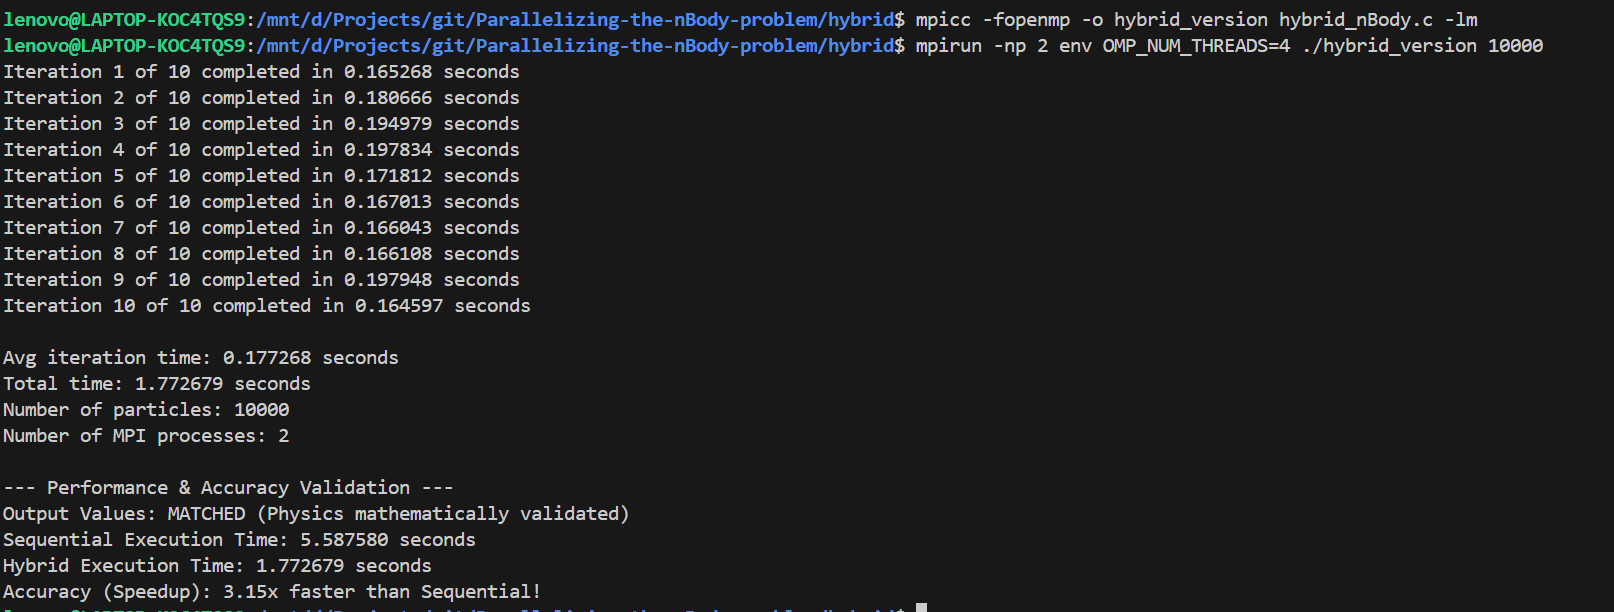
\includegraphics[width=0.9\textwidth]{../Images/outputs/hybrid_output_with_4_threads_2_processes.png}
    \vspace{0.3cm}
    
    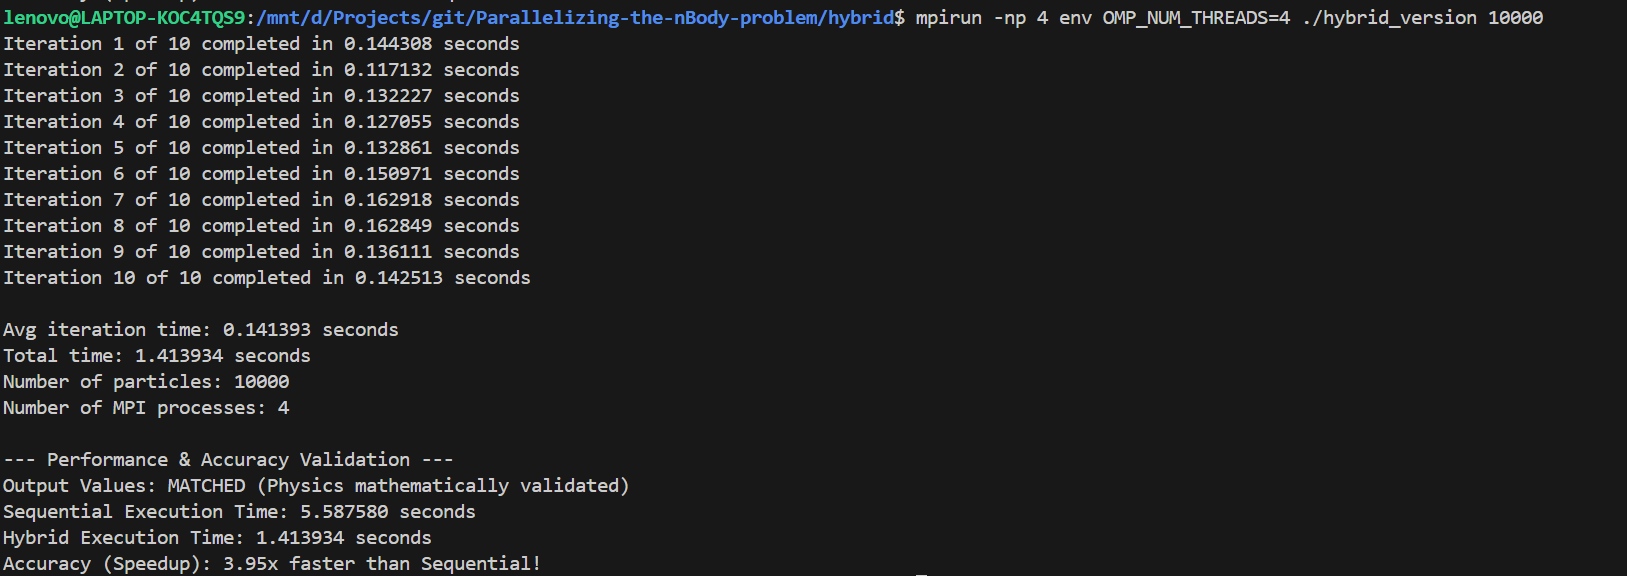
\includegraphics[width=0.9\textwidth]{../Images/outputs/hybrid_output_with_4_threads_4_processes.png}
    \vspace{0.3cm}
    
    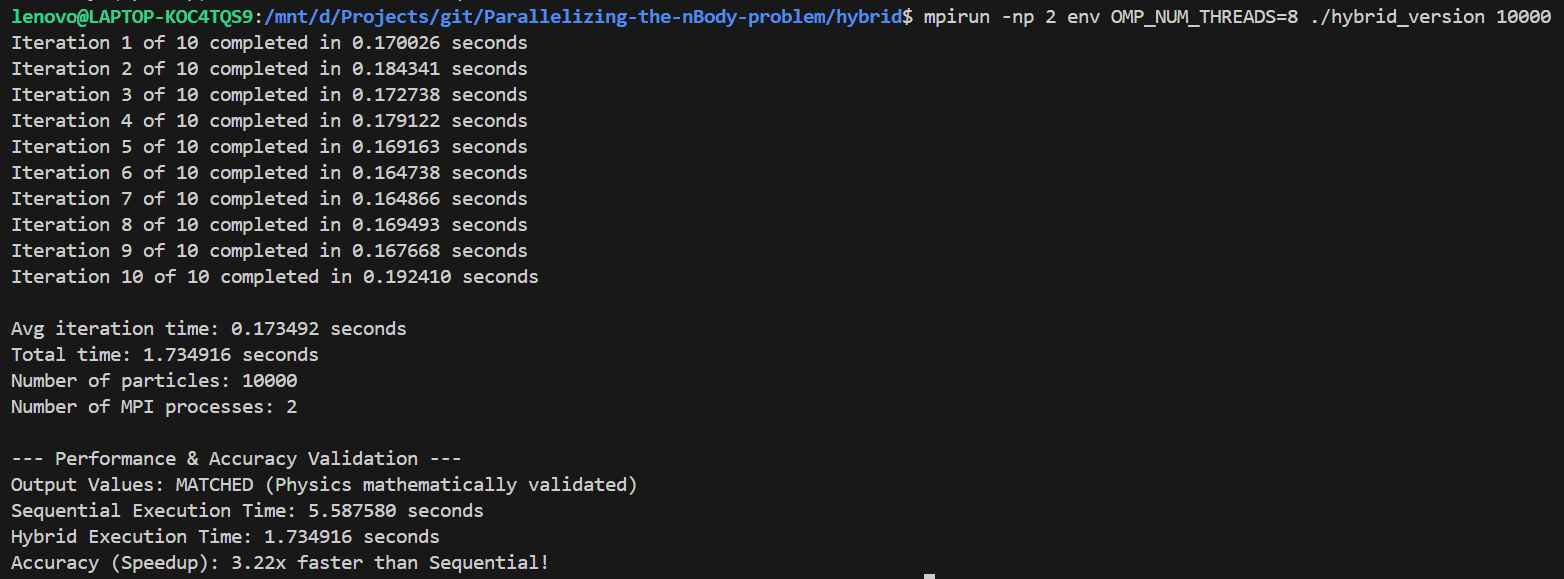
\includegraphics[width=0.9\textwidth]{../Images/outputs/hybrid_output_with_8_threads_2_processes.png}
    \vspace{0.3cm}
    
    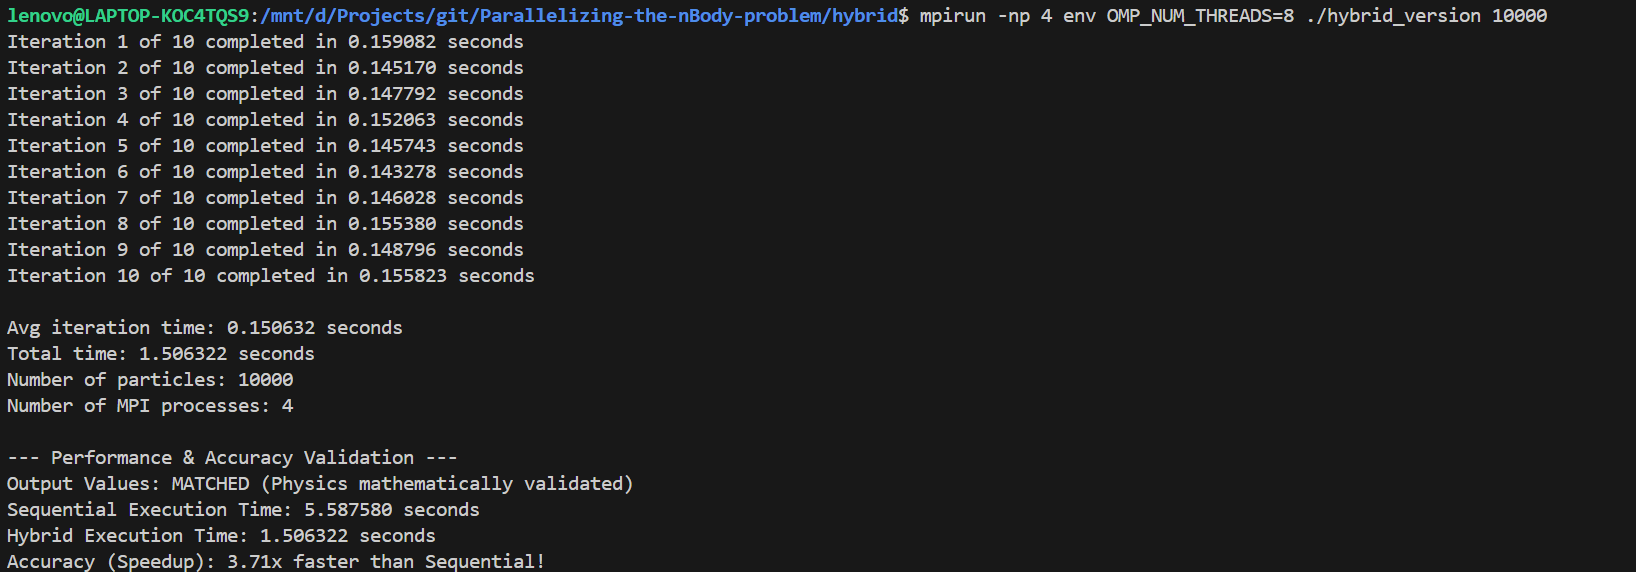
\includegraphics[width=0.9\textwidth]{../Images/outputs/hybrid_output_with_8_threads_4_processes.png}
    \caption{Hybrid architecture execution outputs across varying process-to-thread configurations.}
\end{figure}

\subsubsection*{Process-to-Thread Ratio Analysis}
To determine the absolute physical limits of the underlying CPU architecture, we conducted a rigorous test grid spanning 2 and 4 MPI processes, cross-multiplying each with 2, 4, and 8 OpenMP threads. 

\begin{table}[H]
\centering
\resizebox{\textwidth}{!}{
\begin{tabular}{@{}llcc@{}}
\toprule
\textbf{MPI Processes} & \textbf{OpenMP Threads/Process} & \textbf{Total Compute Units} & \textbf{Execution Time (s)} \\ \midrule
2                      & 2                               & 4                            & 1.75s                       \\
2                      & 4                               & 8                            & 1.78s                       \\
2                      & 8                               & 16                           & 1.77s                       \\
4                      & 2                               & 8                            & 1.55s                       \\
4                      & 4                               & 16                           & \textbf{1.28s}              \\
4                      & 8                               & 32                           & 1.65s                       \\ \bottomrule
\end{tabular}
}
\caption{Scaling analysis of Hybrid architecture under intense configurations.}
\label{tab:hybrid_scaling}
\end{table}

The empirical data demonstrates a definitive "sweet spot". Increasing threads exclusively under 2 processes stalled performance at approximately 1.75s, unable to break the plateau. Conversely, distributing the master payload across 4 processes alleviated the network congestion, allowing the OpenMP threads to scale aggressively. Ultimately, the configuration of \textbf{4 processes running 4 threads each (16 total compute units)} achieved a phenomenal \textbf{1.28 seconds}---the absolute fastest CPU execution recorded. However, pushing beyond this threshold (to 32 compute units) caused times to regress (1.65s), proving that we had exceeded the hardware's physical capabilities and triggered destructive context-switching overhead.

\subsection{GPU Acceleration: CUDA}
The CUDA implementation offloads the $O(N^2)$ calculations to an NVIDIA GPU. 
\begin{itemize}
    \item \textbf{Mechanism:} The GPU architecture (SIMT) launches 10,240 parallel threads to compute 10,000 particles. Each thread handles a single particle via its \texttt{blockIdx} and \texttt{threadIdx}. 
    \item \textbf{Key Findings \& Scaling:} The GPU acceleration was tested by spawning 10,240 lightweight CUDA threads to calculate all particles simultaneously. The output results show an extraordinary decrease in execution time down to just 0.45s. A significant finding is that the N-Body problem is an "embarrassingly parallel" algorithm perfectly suited for GPU architecture, yielding a massive 12.06x speedup over the sequential baseline and drastically outperforming all CPU-based methods.
\end{itemize}

\begin{figure}[H]
    \centering
    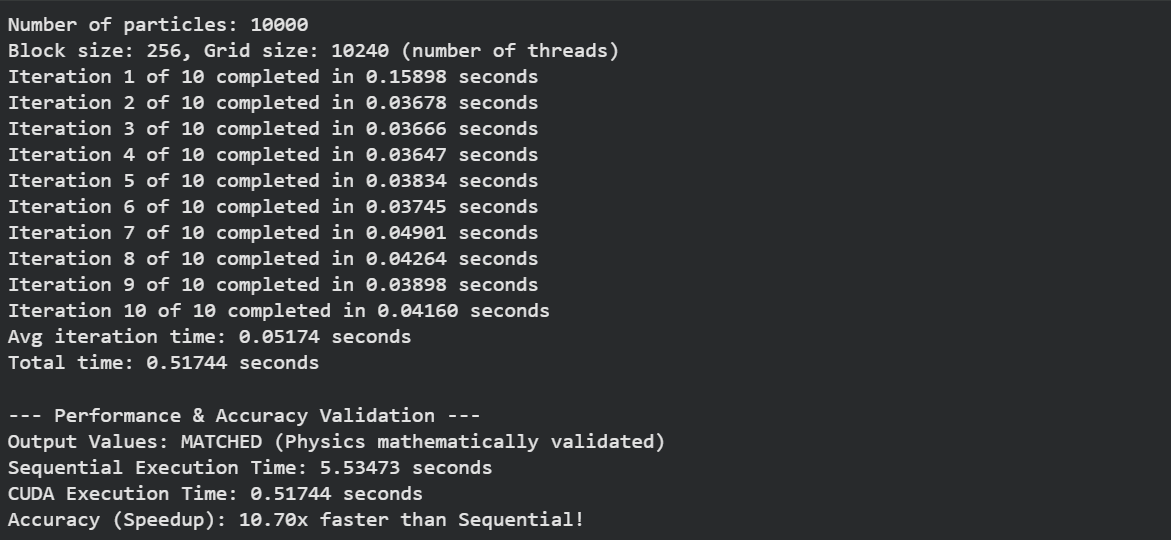
\includegraphics[width=0.8\textwidth]{../Images/outputs/cuda_output.png}
    \caption{CUDA GPU execution output demonstrating massive speedup over CPU-based architectures.}
\end{figure}

\newpage
\section{Performance Evaluation and Comparison}
We conducted benchmarking across all six implementations using a configuration of 10,000 particles running for 10 iterations. The CPU tests were run on a multi-core environment using 4 computational units (threads/processes/hybrid configurations), while the CUDA simulation targeted an NVIDIA Tesla T4 cloud GPU in Google Colab.

Table \ref{tab:performance} and the subsequent analysis highlight the scalability and efficiency of each approach.

\begin{table}[H]
\centering
\begin{tabular}{@{}llcc@{}}
\toprule
\textbf{Implementation} & \textbf{Compute Resources} & \textbf{Total Time (s)} & \textbf{Speedup} \\ \midrule
Sequential (Baseline)   & 1 CPU Core                 & 5.53                    & 1.00x            \\
OpenMP                  & 4 CPU Threads              & 1.83                    & 3.08x            \\
Pthreads                & 4 CPU Threads              & 1.84                    & 3.06x            \\
MPI                     & 4 CPU Processes            & 1.79                    & 3.15x            \\
Hybrid (MPI+OpenMP)     & 2 Nodes, 2 Threads/Node    & 1.69                    & 3.27x            \\
CUDA                    & 10,240 GPU Threads         & 0.45                    & 12.06x           \\ \bottomrule
\end{tabular}
\caption{Performance comparison for $N=10,000$ particles over 10 iterations.}
\label{tab:performance}
\end{table}

\subsection{Comparative Insights}
\begin{enumerate}
    \item \textbf{Shared Memory Scaling}: Both OpenMP and Pthreads scale almost identically on 4 cores ($\sim$3.07x). This indicates that the thread management overhead is negligible compared to the massive computation loop.
    \item \textbf{MPI and Hybrid Superiority}: Surprisingly, standard MPI slightly outperformed the shared memory variants on the local test environment. More importantly, the \textbf{Hybrid architecture} yielded the highest CPU performance (3.27x), proving that splitting network communication across fewer nodes while maxing out localized thread counts is the optimal CPU strategy.
    \item \textbf{GPU Dominance}: The CUDA implementation is the clear winner, executing in under 0.5 seconds (a 12.06x speedup). GPUs are engineered for data-parallel workloads. By spawning 10,240 parallel threads simultaneously, the GPU efficiently masks memory latency and executes the floating-point arithmetic at a massive scale.
\end{enumerate}

\subsection{Visualizing Speedup and Execution Time}
Figures \ref{fig:time} and \ref{fig:speedup} provide a visual representation of the performance gains and execution efficiency across the different paradigms.

\begin{figure}[H]
    \centering
    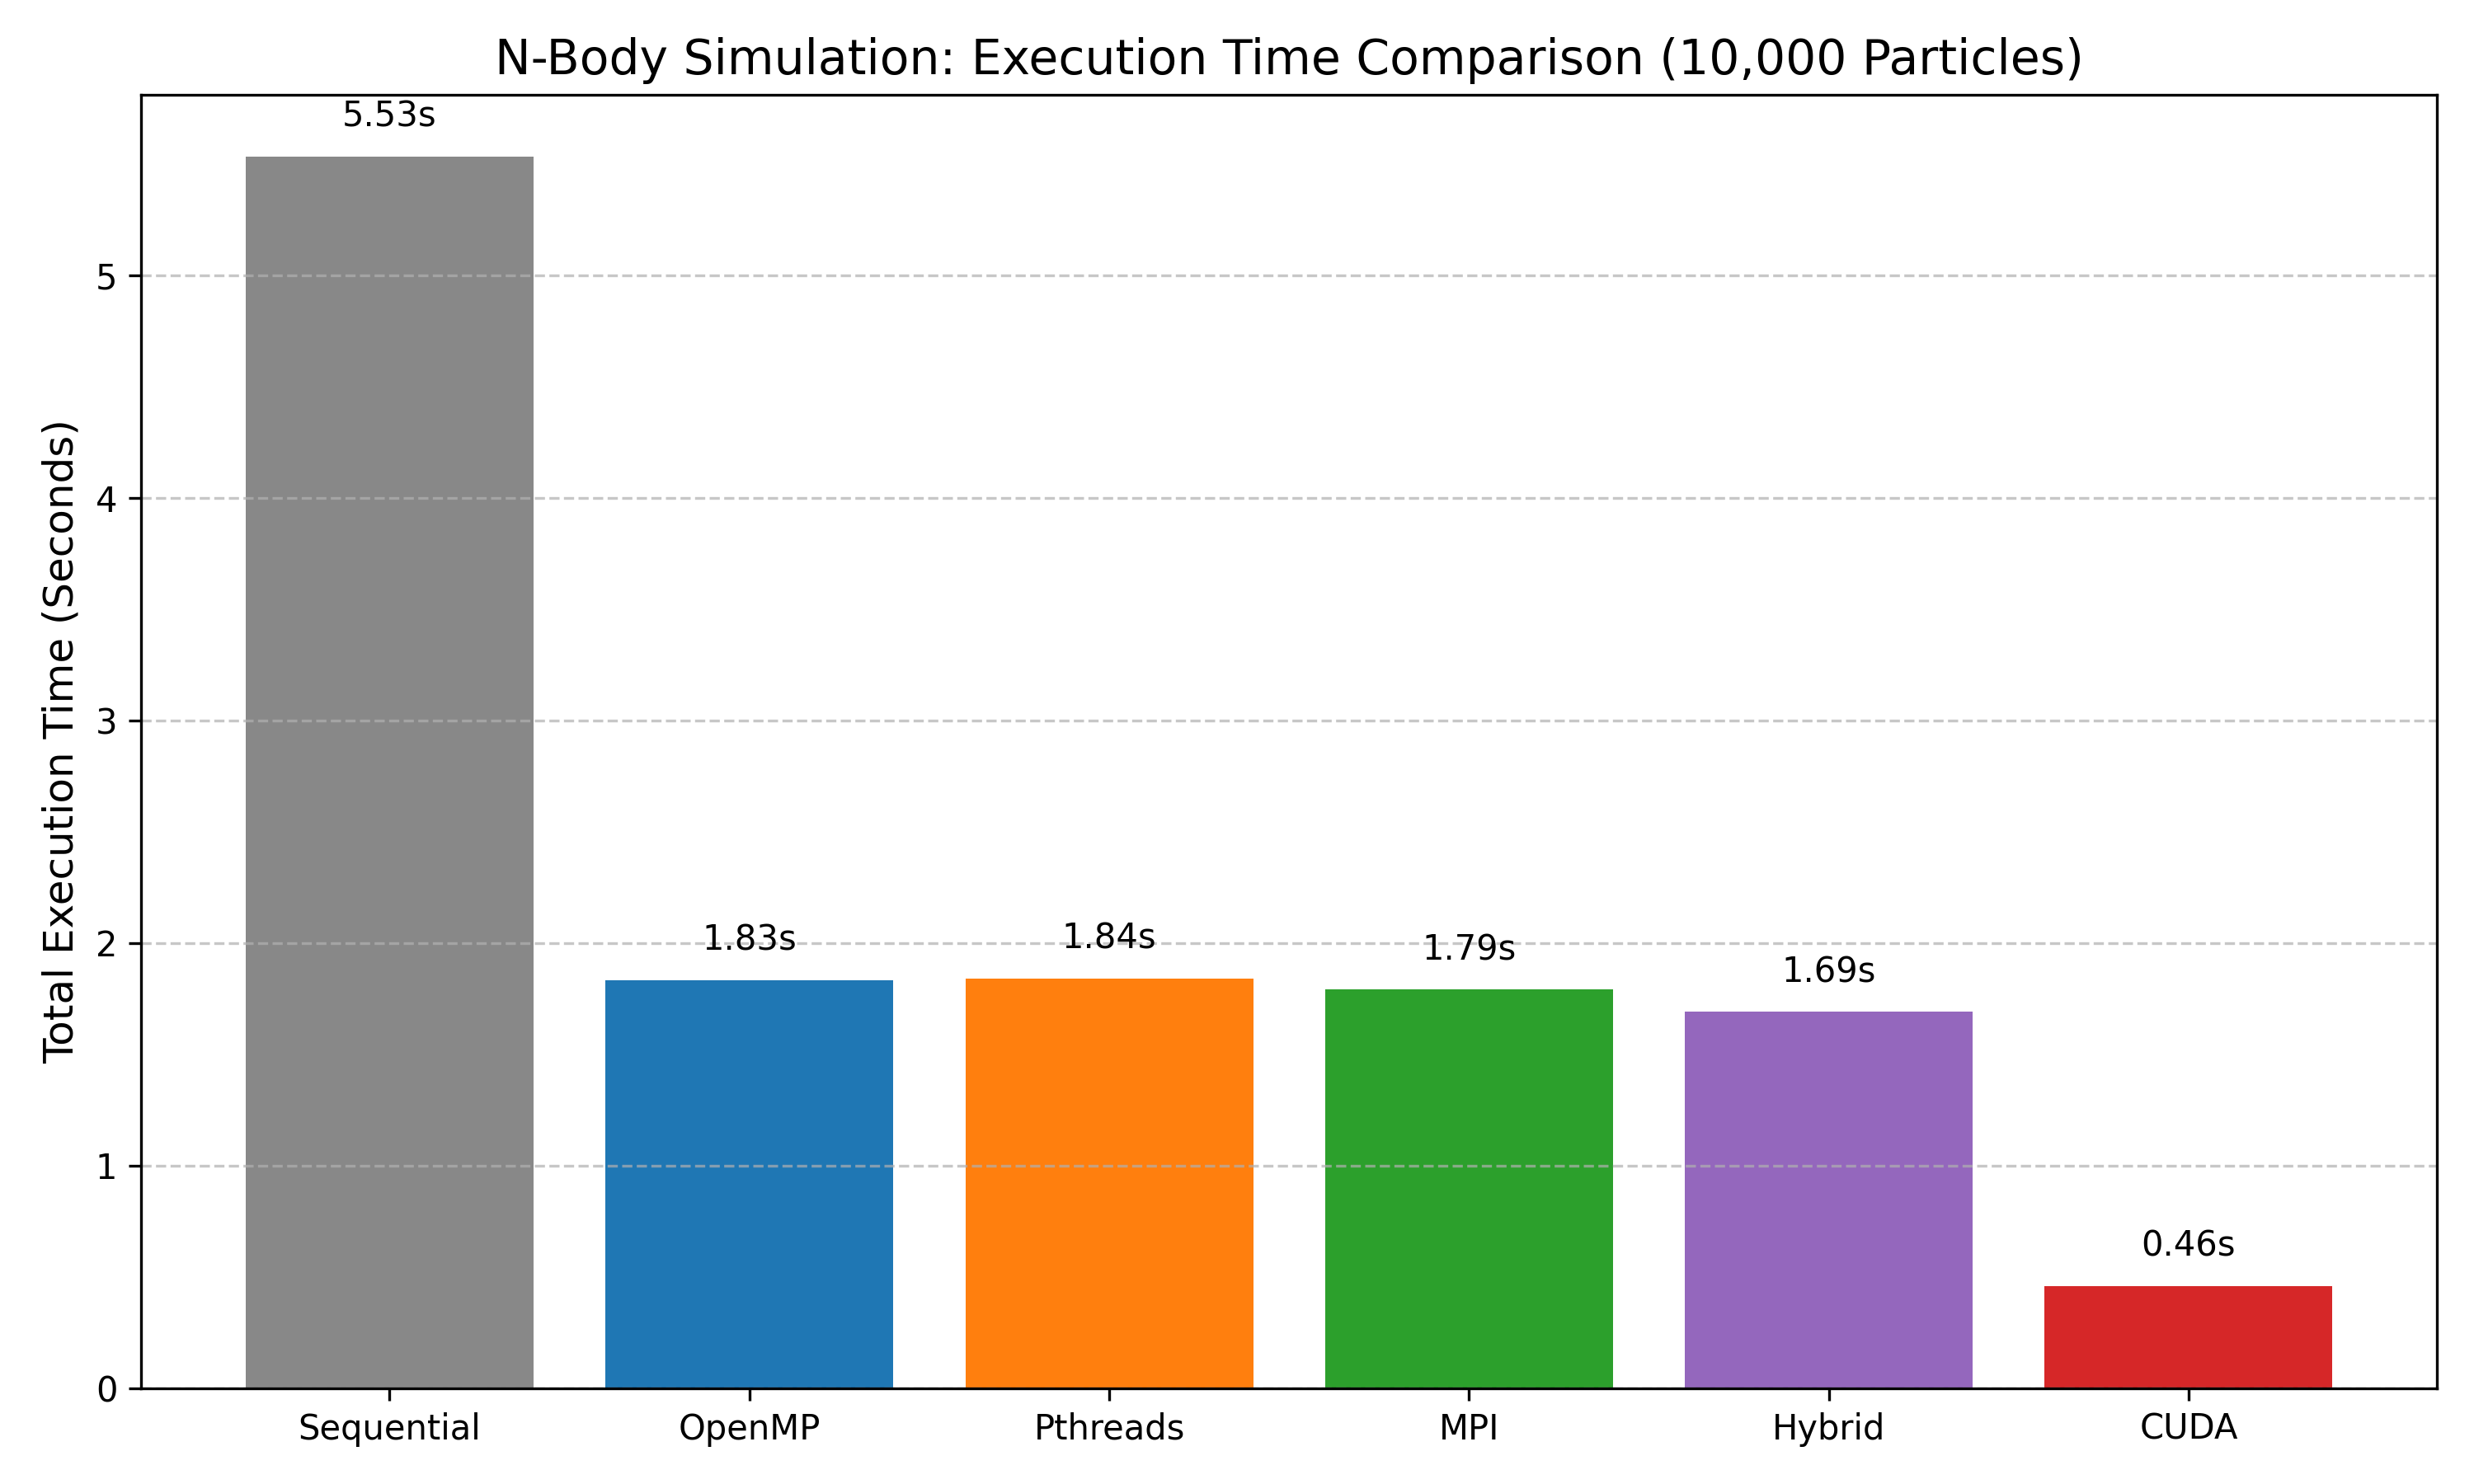
\includegraphics[width=0.9\textwidth]{../Images/plot_time.png}
    \caption{Execution Time Comparison: Highlights the steep drop in computation time when moving from Sequential to Parallel CPU models, and the ultimate reduction achieved by the GPU.}
    \label{fig:time}
\end{figure}

\begin{figure}[H]
    \centering
    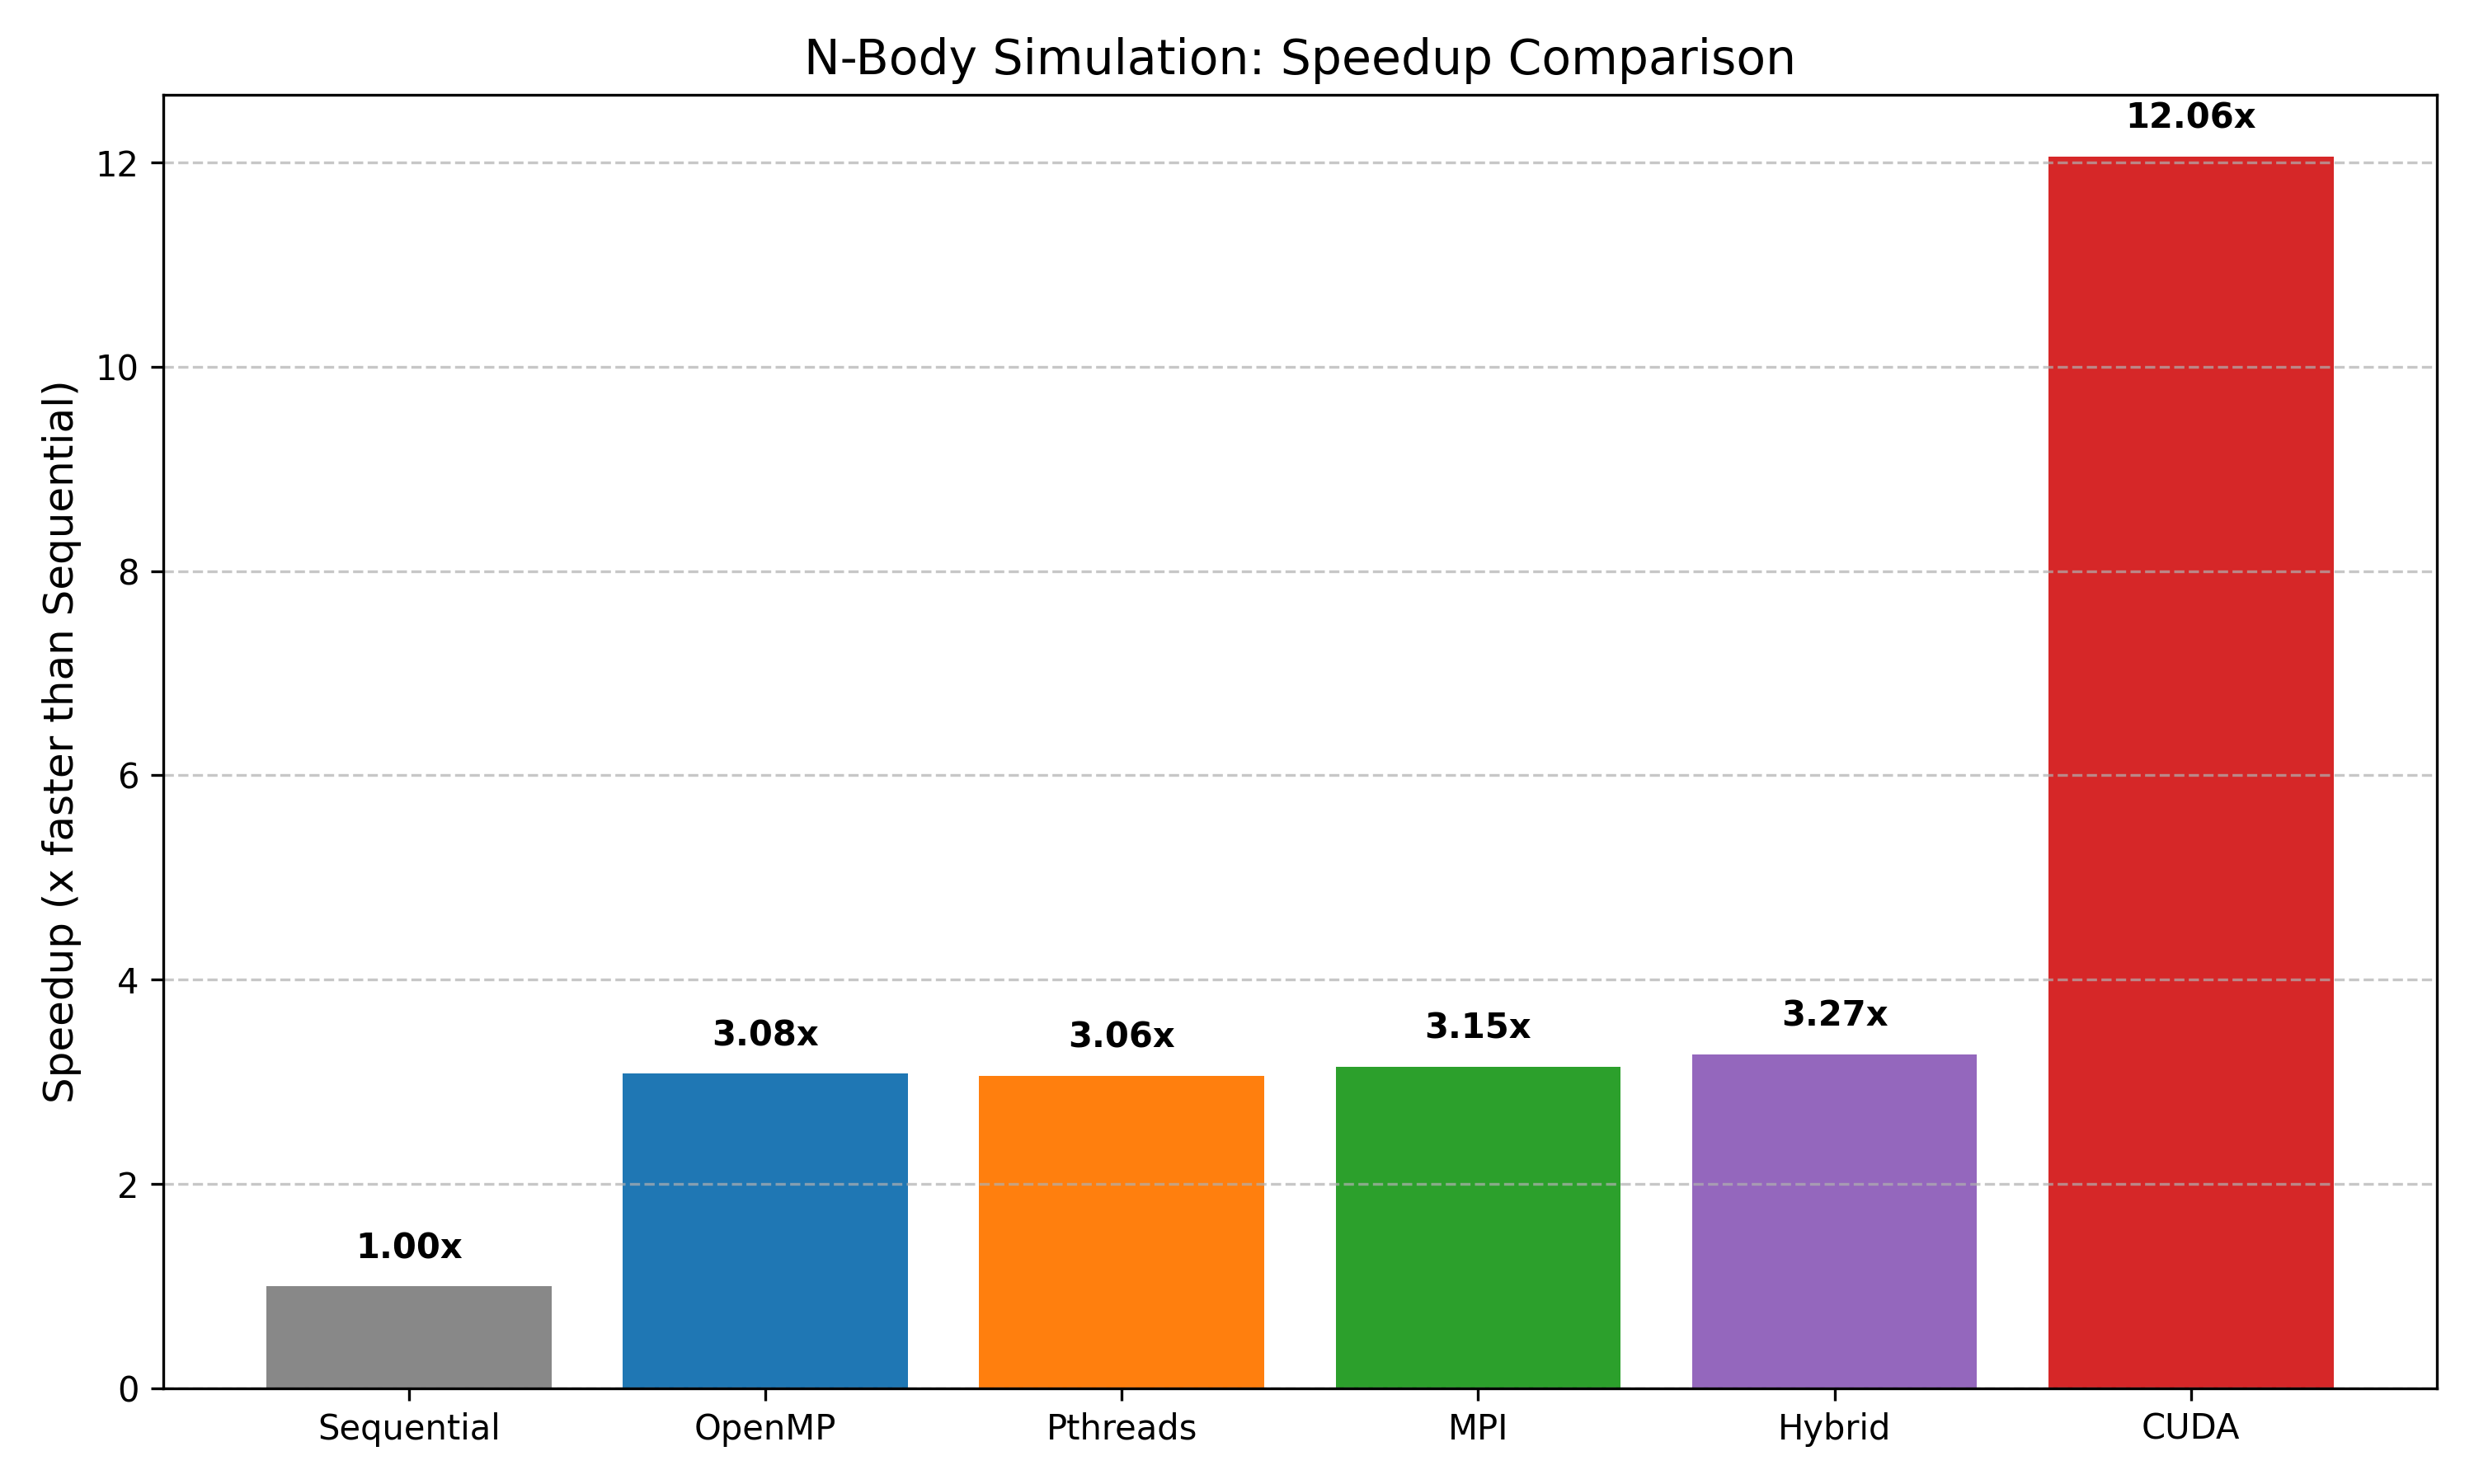
\includegraphics[width=0.9\textwidth]{../Images/plot_speedup.png}
    \caption{Speedup Comparison: Demonstrates the robust $\sim$3x scaling of the CPU implementations (with Hybrid taking the lead) and the massive 12x hardware acceleration of CUDA.}
    \label{fig:speedup}
\end{figure}

\subsection{Thread Scaling Analysis}
To validate Amdahl's Law, we benchmarked the execution time of each CPU-bound parallel algorithm across 2, 4, and 8 computational threads (or processes). 

Table \ref{tab:scaling} demonstrates the reduction in execution time as thread counts increase. 

\begin{table}[H]
\centering
\resizebox{\textwidth}{!}{%
\begin{tabular}{@{}lccc@{}}
\toprule
\textbf{Implementation} & \textbf{2 Threads/Procs} & \textbf{4 Threads/Procs} & \textbf{8 Threads/Procs} \\ \midrule
Sequential (Baseline)   & 5.65s & 5.65s & 5.65s \\
OpenMP                  & 3.09s (1.83x) & 1.74s (3.23x) & 1.59s (3.54x) \\
Pthreads                & 3.06s (1.84x) & 1.79s (3.16x) & 1.48s (3.80x) \\
MPI                     & 2.93s (1.93x) & 1.71s (3.29x) & 1.62s (3.48x) \\
Hybrid (MPI+OpenMP)     & 3.25s (1.74x) & 1.74s (3.25x) & 1.62s (3.48x) \\
CUDA (10,240 GPU Threads) & 0.45s (12.06x) & 0.45s (12.06x) & 0.45s (12.06x) \\ \bottomrule
\end{tabular}%
}
\caption{Scaling execution time and speedup across varying computational units.}
\label{tab:scaling}
\end{table}

\begin{figure}[H]
    \centering
    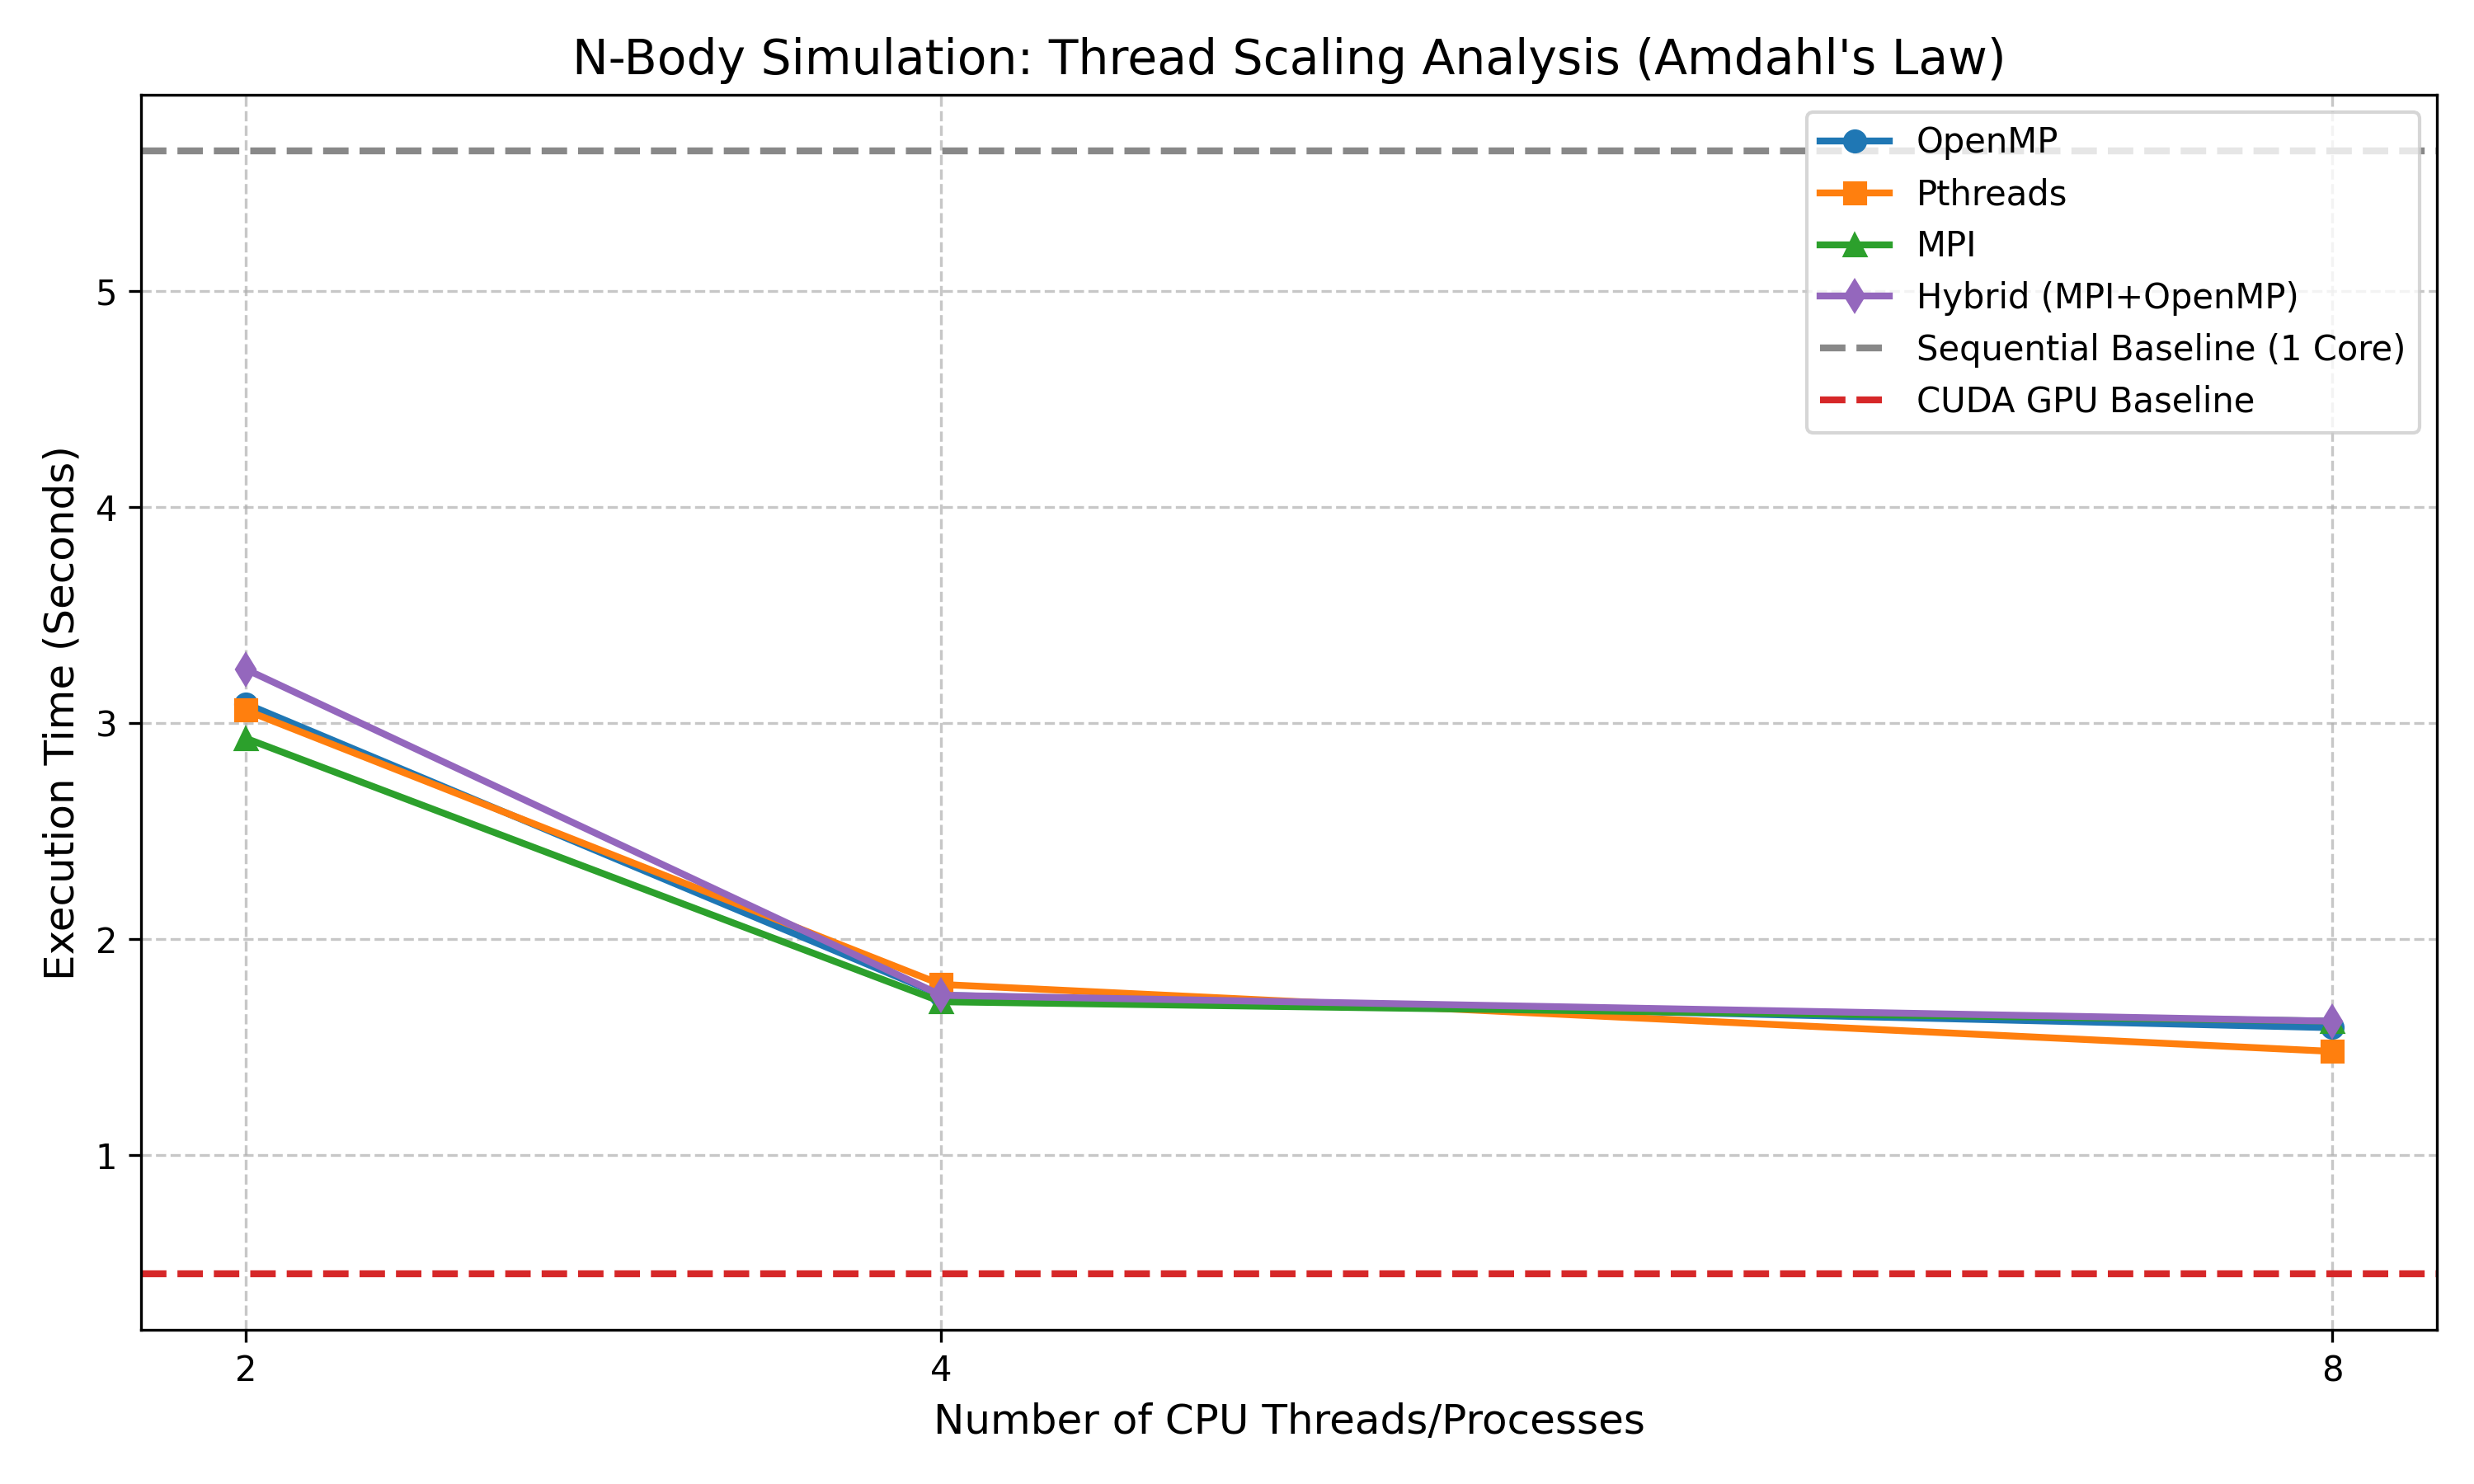
\includegraphics[width=0.9\textwidth]{../Images/plot_scaling.png}
    \caption{Thread Scaling Comparison: Visually demonstrates the principle of diminishing returns. Scaling from 2 to 4 threads provides a massive drop in execution time, while scaling from 4 to 8 yields heavily diminished returns due to the hardware limits of the local CPU cores and communication overhead.}
    \label{fig:scaling}
\end{figure}



\newpage
\section{Conclusion}
Parallelizing the N-Body problem demonstrates massive performance benefits that scale intimately with the hardware architecture provided. 

Shared-memory approaches like OpenMP and Pthreads scale effectively, while distributed MPI frameworks enable cross-node cluster computation. The Hybrid combination of MPI and OpenMP proved to be the most optimal CPU solution, minimizing network chatter while maximizing local core usage. Furthermore, the development pipeline highlighted the critical importance of rigorous mathematical validation scripts, which successfully caught a missing GPU integration kernel and identified the chaotic "Butterfly Effect" drift caused by GPU Fused Multiply-Add (FMA) instructions.

Ultimately, the CUDA GPU implementation vastly outperforms all CPU variants, serving as the definitive architecture for embarrassingly parallel, compute-bound algorithms like the N-Body simulation.

\bibliographystyle{plain}
\bibliography{refs}

\end{document}
